\newcommand{\ptab}{\hspace*{0.5cm}}

\newcommand{\spinlockLib}{
  $\kw{void}\ lock(l)\ \{$ \\
  \ptab $\kw{repeat}\ \{\}$ \\
  \ptab $\kw{until}\ CAS(l, 0, 1);$ \\
  $\}$ \\
  
  $\kw{void}\ unlock(l)\ \{$\\
  \ptab$\writeInst{l}{0};$\\
  $\}$
}

\newcommand{\spinlockClientII}{
  \begin{figure}[h]
    \centering
    \begin{tabular}{l | l}
      \multicolumn{2}{c}{$\writeInst{l}{0}{}$} \\
      \hline
      $lock(l);$ & $lock(l);$ \\
      $unlock(l);$ & $unlock(l);$ \\
    \end{tabular}
  \end{figure}    
}
\newcommand{\spinlockClientIICS}{
  \begin{figure}[h]
    \centering
    \begin{tabular}{l | l}
      \multicolumn{2}{c}{$\writeInst{l}{0}{}$} \\
      \hline
      $lock(l);$ & $lock(l);$ \\
      $\comment{critical section}$ & $\comment{critical section}$ \\
      $unlock(l);$ & $unlock(l);$ \\
    \end{tabular}
  \end{figure}    
}

\newcommand{\spinlockClientIIExtSep}{
  \begin{figure}[h]
    \centering
    \begin{tabular}{p{3cm} || p{3cm}}
      \multicolumn{2}{c}{$\writeInst{l_1}{0}{}; \writeInst{d_1}{0}{}; \writeInst{l_2}{0}{}; \writeInst{d_2}{0}{};$} \\
      \hline
      $lock(l_1);$ & $lock(l_2);$ \\
      $\readInst{r}{d_1};$ & $\readInst{r}{d_2};$ \\
      $\writeInst{d_1}{r + 1};$ & $\writeInst{d_2}{r + 1};$ \\
      $unlock(l_1);$ & $unlock(l_2);$ \\
    \end{tabular}
  \end{figure}    
}

\newcommand{\spinlockLibClientII}{
  \begin{minipage}[c]{0.25\linewidth}
    \spinlockLib
  \end{minipage}
  \begin{minipage}[c]{0.25\linewidth}
    \spinlockClientII
  \end{minipage}
}
\newcommand{\spinlockLibClientIIVert}{
  \begin{minipage}[c]{0.25\linewidth}
    \spinlockLib
    \vspace{-0.5cm}
    \spinlockClientII
  \end{minipage}
}

\newcommand{\spinlockClientIIExpanded}{
  \begin{figure}[h]
    \centering
    \begin{tabular}{l | l}
      \multicolumn{2}{c}{$\writeInst{l}{0}{}$} \\
      \hline
      % $\kw{while}\ (\neg CAS(l, 0, 1)) \{\};$ & $\kw{while}\ (\neg CAS(l, 0, 1)) \{\};$ \\
      % $\kw{while}\ (\neg CAS(l, 0, 1))$ & $\kw{while}\ (\neg CAS(l, 0, 1))$ \\
      % $\qquad \qquad \{\};$ & $\quad \quad \{\};$ \\
      $\kw{repeat}\ \{\}$ & $\kw{repeat}\ \{\}$ \\
      $\kw{until}\ CAS(l, 0, 1);$ & $\kw{until}\ CAS(l, 0, 1);$ \\
      $\comment{critical section}$ & $\comment{critical section}$ \\
      $\writeInst{l}{0};$ & $\writeInst{l}{0};$ \\
    \end{tabular}
  \end{figure}    
}

\newcounter{evctr}
\newcommand{\curEv}{\theevctr}
\newenvironment{traceenvNoThreads}[2]
{
  \setcounter{evctr}{0}
  \begin{tikzpicture}[xscale=#1, yscale=#2]
}
{
  \node (E1) at (0, 0.5) {}; \node (E2) at (\curEv, 0.5) {};
  % \dpo{E1}{E2};
  \draw[time] (E1) edge node[] { } (E2);
  \end{tikzpicture}
}
\newenvironment{traceenv}[2]
{
  \begin{traceenvNoThreads}{#1}{#2}
}
{
  \node (T1) at (-0.5 * 1, 1) {\textbf{Thread 1}};
  \node (T2) at (-0.5 * 1, 0) {\textbf{Thread 2}};
  \node (timePic) at (\curEv + 0.25, 0.5) {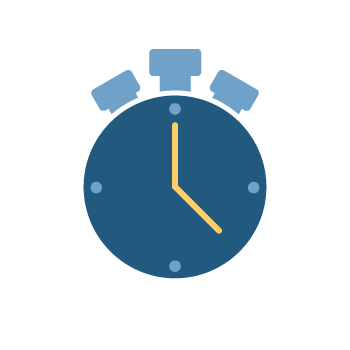
\includegraphics[width=0.1\textwidth]{time.png}};
  \end{traceenvNoThreads}
}



\newcommand{\SCDeclUnfair}{
  \begin{figure}[h]
    \centering
    \begin{tabular}{p{3cm} || p{3cm}}
      \multicolumn{2}{c}{$\writeInst{x}{0}{}$} \\
      \hline
      $\writeInst{x}{1};$ & $\kw{while} (\kw{true})\ \{$ \\
      $\kw{while} (\kw{true})\ \{$ & $\quad \writeInst{x}{2};$ \\
      $\quad \readInst{r}{x};\comment{1,1,\ldots}$ & $\}$ \\
      $\}$ & ${}$ \\
    \end{tabular}
  \end{figure}
}

\newcommand{\SCDeclUnfairEvents}{
  \node (W1) at (0 * \hof, -0 * \vof) {$\evlab{\lW}{}{x}{1}$};
  \node (R11) at (0 * \hof, -1 * \vof) {$\evlab{\lR}{}{x}{1}$};
  \node (R12) at (0 * \hof, -2 * \vof) {$\evlab{\lR}{}{x}{1}$};
  \node (R1inf) at (0 * \hof, -2.5 * \vof) {$\ldots$};

  \node (W21) at (1 * \hof, -0 * \vof) {$\evlab{\lW}{}{x}{2}$};
  \node (W22) at (1 * \hof, -1 * \vof) {$\evlab{\lW}{}{x}{2}$};
  \node (W2inf) at (1 * \hof, -1.5 * \vof) {$\ldots$};
    
  % \dpo{L1}{R1}; \dpo{R1}{W1}; \dpo{W1}{U1}; 
  % \dpo{L2}{R2}; \dpo{R2}{W2}; \dpo{W2}{U2};         
}


\newcommand{\spinlockInfGraphEvents}{      
      \node (U1) at (0 * \hof, -0 * \vof) {$\evlab{\lU}{}{l}{0, 1}$};
      \node (W1) at (0 * \hof, -2 * \vof) {$\evlab{\lW}{}{l}{0}$};

      \node (R21) at (1 * \hof, -0 * \vof) {$\evlab{\lR}{}{l}{1}$};
      \node (R22) at (1 * \hof, -2 * \vof) {$\evlab{\lR}{}{l}{1}$};
      \node (R23) at (1 * \hof, -4 * \vof) {$\evlab{\lR}{}{l}{1}$};
      \node (R24) at (1 * \hof, -5 * \vof) {$\ldots$};
}
\newcommand{\spinlockInfGraphPO}{
      \dpo{U1}{W1};
      \dpo{R21}{R22}; \dpo{R22}{R23};
}
\newcommand{\spinlockInfGraphRF}{
      \node (W0) at (0.5 * \hof, 1 * \vof) {$\evlab{\lW}{}{l}{0}$};
      \drf{W0}{U1};
      \drf{U1}{R21}; \drf{U1}{R22}; \drf{U1}{R23};
}
\newcommand{\spinlockInfGraphMO}{
      \dmo[bend left=30]{W0}{U1}; \dmo[bend right=30]{U1}{W1};
}
% \newcommand{\spinlockInfGraphFRComp}{
%   \draw[frComp,bend right=60] (R21) edge node[] { } (W1);
%   \draw[frComp,bend right=60] (R22) edge node[] { } (W1);
%   \draw[frComp,bend right=120] (R23) edge node[] { } (W1);
% }
\newcommand{\spinlockInfGraphRB}{
  % \draw[fr,bend right=60] (R21) edge node[] { } (W1);
  % \draw[fr,bend right=60] (R22) edge node[] { } (W1);
  % \draw[fr,bend right=120] (R23) edge node[] { } (W1);
  \dfr{R21}{W1}{bend right=20};
  \dfr{R22}{W1}{bend right=30};
  \dfr{R23}{W1}{};
}
\newcommand{\spinlockInfGraphComments}{
      \node (V1) at (0.5, -4) {}; \node (V2) at (1.5, -4) {};
      \draw[po] (V1) edge node[yshift=0.2cm, right] { } (V2);
      \node at (1, -4.5) {``program order''};      
}

\newcommand{\spinlockContraGraphEventsI}{
  \node (W0) at (0.5 * \hof, 1 * \vof) {$\evlab{\lW}{}{l}{0}$};
  \node (U1) at (0 * \hof, -0 * \vof) {$\evlab{\lU}{}{l}{0, 1}$};
  \node (W1) at (0 * \hof, -2 * \vof) {$\evlab{\lW}{}{l}{0}$};

  \node (R21) at (1 * \hof, -0 * \vof) {$\evlab{\lR}{}{l}{1}$};
  \node (R22) at (1 * \hof, -2 * \vof) {$\evlab{\lR}{}{l}{1}$};
  \node (R23) at (1 * \hof, -3 * \vof) {$\ldots$};
}
\newcommand{\spinlockContraGraphEventsII}{
  \node (R24) at (1 * \hof, -4 * \vof) {$\evlab{\lR}{}{l}{0}$};
  \node (R25) at (1 * \hof, -5 * \vof) {$\ldots$};
  
}
\newcommand{\spinlockContraGraphRelationsI}{
      \dpo{U1}{W1};
      \dpo{R21}{R22}; 

      \drf{U1}{R21}; \drf{U1}{R22};
      \dmo[bend left=30]{W0}{U1}; \dmo[bend right=30]{U1}{W1};

      \dfr{R21}{W1}{}; \dfr{R22}{W1}{};
}
\newcommand{\spinlockContraGraphRelationsII}{
  \drf{W1}{R24};
  \node (coqPic) at (0.75 * \hof, -4 * \vof) {{\LARGE $\exists$}};  
}
\newcommand{\spinlockContraGraphContra}{
  \node (Contra) at (1.2 * \hof, -4.5 * \vof) {{\color{red} \LARGE ?!}};
}
 
    
\newcommand{\propSubtrace}{
  \begin{traceenvNoThreads}{1.0}{0.9}
    \stepcounter{evctr}
    % \node (dummy) at (0, 2) {};
    \node at (\curEv, 1) {$\ldots$ \stepcounter{evctr}};
    \node at (\curEv, 1) {\color{blue} \underline{$\mathtt{prop}$} \stepcounter{evctr}};
    \node at (\curEv, 0) {$\ulab{}{l}{0}{1}$ \stepcounter{evctr}};
    \node at (\curEv, 0) {$\ldots$ \stepcounter{evctr}};
  \end{traceenvNoThreads}
}
    
\newcommand{\mmEquiv}[2]{
  $#1 = #2 \cap \fairDecl$
}
\newcommand{\tsoEquiv}{\mmEquiv{\TSOopfair}{\TSOdecl}}

%%% Local Variables:
%%% mode: latex
%%% TeX-master: "oopsla"
%%% End:
